\RequirePackage{snapshot}
\documentclass [10pt, fancyhdr, twoside] {article}
\usepackage{float, graphicx, caption, amssymb, natbib}
\usepackage[usenames,dvipsnames]{color}
\usepackage{tabulary}
\usepackage [left=2.5cm, top=2.5cm, bottom=2.5cm, right=3cm] {geometry}  %% see geometry.pdf on how to lay out the page. There's lots.
\geometry{a4paper} %% or letter or a5paper or ... etc
\usepackage{fancyhdr}
\usepackage{xcolor}
\usepackage[scaled]{helvet}
\usepackage{tcolorbox}
\renewcommand*\familydefault{\sfdefault} %% Only if the base font of the document is to be sans serif

\usepackage[left]{lineno}
\usepackage[yyyymmdd,hhmmss]{datetime}

\renewcommand{\linenumberfont}{\normalfont\tiny\color{gray}}
\usepackage{enumitem}
\usepackage{bbding}
\usepackage{tikz}

\pagestyle{fancy}

\fancyhf{}

%\fancyhead[RO,LE]{Heading}
%\fancyfoot[RO,LE]{}
\fancyfoot[C]{\thepage}
%\fancyfoot[RE, LO]{}

%\sectionfont{\centering}
%\subsectionfont{\centering}
\setcounter{secnumdepth}{0}

\usepackage{blindtext}

\newcounter {note}
\stepcounter{note}

\renewcommand{\abstractname}{Abstract Name}

\newcommand {\Note} [1] {
    \marginpar {
        \tiny {
            {\color{gray}{\thenote  \  #1}}
            }
        }
    \stepcounter {note}
}

\newcommand {\MNote} [1] {
    \marginpar {
        \tiny {
            {\color{gray}{#1 }}
            }
        }
}

\begin{document}

\title{Analýza \textsc{Cash Flow} \\
  \large Účetně kompatibilní metoda pro hodnotový management \\
}


\author{
  Ing. Karel Hubálek, CSc.
  \and
  RNDr. Edvard Špaček
}
\date{}


\maketitle

\newcommand\HRule{\rule{\textwidth}{1pt}}

\begin{center}

\HRule \\[0.4cm]
{ \huge \bfseries \textsc{\LARGE Vesna 3}}\\[0.4cm]

\HRule \\[2cm]

\end{center}

\section{Nabídka rozšíření metody}

Při zachování principu hodnocení efektivnosti akci metodou \textsc{Vesna} 1 a 2 tento modul umožňuje vycházet z účetní bilance dané výkazy Výsledovka, Rozvaha a Tok hotovosti.

Metoda \textsc{Vesna} 3 transformuje data z účetních výkazů alternativně do formy podnikatelstkého záměru pro vyhodnocení metodou \textsc{Vesna} 1 a 2. Tak provazuje účetní evidenci podnikatelských akcí s splněním požadavků na efektivnost dílčí akce a vlivem na celopodnikovou efektivnost.


\section{Co metoda přináší}

\begin{itemize}[label=\NibRight]
\item Návrh a analýza podnikatelstkého záměru zadaný formou účetně návazných dokladů.
\item Propočítá různé způsobý financování, bonitu a další podílové ukazatele podniku s jejich vlivem na finanční řízení.
\item Stanovuje progresivnost akce z hlediska hospodaření s aktivy a pasivy i ziskovosti.
\item Rezultuje do toku hotovosti.
\item Pro detailní rozpis dílčích složek cash flow a jeho charakteristiky se váže na VESNU 1.
\end{itemize}

\subsection{Další přístupy uplatněné v metodě \textsc{Vesna} 3}

Ve výpočtu se získají podílové ukazatele, které jsou v podnikovém řízení všeobecně uplatňovány, zejména:

\begin{itemize}
\item Likvidita (schopnost plnit závazky)
\item Výkonost aktiv (hospodaření s aktivy po stránce tržeb)
\item Marže zisku (ziskovost)
\end{itemize}

\subsection{Postup výpočtu}

\begin{enumerate}
\item Uživatel vyplní při zádání vstupů tabulky \textbf{Výsledovka, Rozvaha a Tok hotovosti}.
\item Počítač vypíše tabulku \textbf{Vybrané ukazatele pro finanční řízení} (tab. 1 a 2). Podává přehled o hlavních parametrech akce. Dále vypíše sestavu \textbf{Podílové ukazatele pro fin. řízení} (tab. 4). Podává přehled o kriteriálních ukazatelích. Tyto porovnává s normativy a stanovuje s pomocí vah celkové hodnocení bonity.

\pagebreak

Dalšími vstupními sestavami jsou:

\begin{itemize}
\item tabulky Výsledovka, Rozvaha, Tok hotovosti (Opis)
\item diagram Podílové ukazatele - přehled (obr. 1)
\item diagram Hodnocení výsledků (obr. 2)
\item diagram Analýza splátek a úroku
\item diagram Analýza splátek leasingu
\item diagram Propočet odpisů (tab. 3)
\item diagram Vývoj aktiv a pasiv (obr. 3)
\item diagram Podíly ukazatelů na výsledcích
\item diagram Diskontovaný cash flow (obr. 4)
\item diagram Skladba celkového výnosu (obr. 5)
\end{itemize}

\item Pro snažší vyplnování základních vstupních podkladů je k dispozici varianta \textsc{Zadávání pomocí trendů a normativů} s uplatněním \textbf{trendového vývoje} vstupních ukazatelů a vyplněním pouze 1. roku průběhu akce. Zde se vyplní vstupní tabulky Výsledovka, Rozvaha a Tok hotovosti s ukazateli pouze pro první rok a jejich meziroční trend.

To umožňuje tvořit podnikatelský záměr interaktivním způsobem na základě různých variant vývoje aktiv, pasiv, investičního majetku, financování a zisku.

\end{enumerate}


\begin{tcolorbox}
\textbf{Metodou \textsc{Vesna} 3 získáte efektivností podložené podnikatelstké plány, navíc s přímou vazbou na účetní výkazy.} Tím se uzavře zpětný okruh přes efektivnost dílčích podnikatelských akcí k hospodaření podniku jako celku!
\end{tcolorbox}


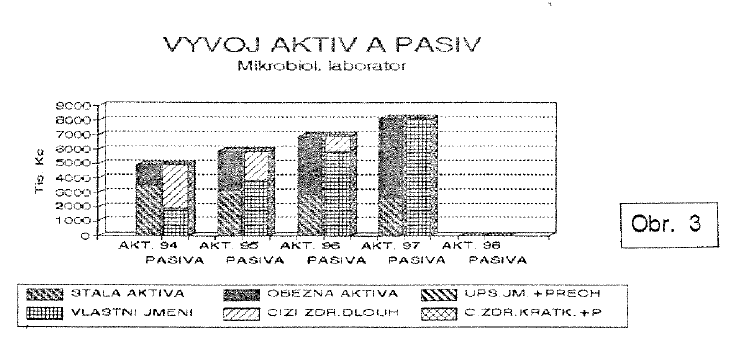
\includegraphics[width=\textwidth,height=\textheight,keepaspectratio]{./vesna3-obr1.png}

\newpage

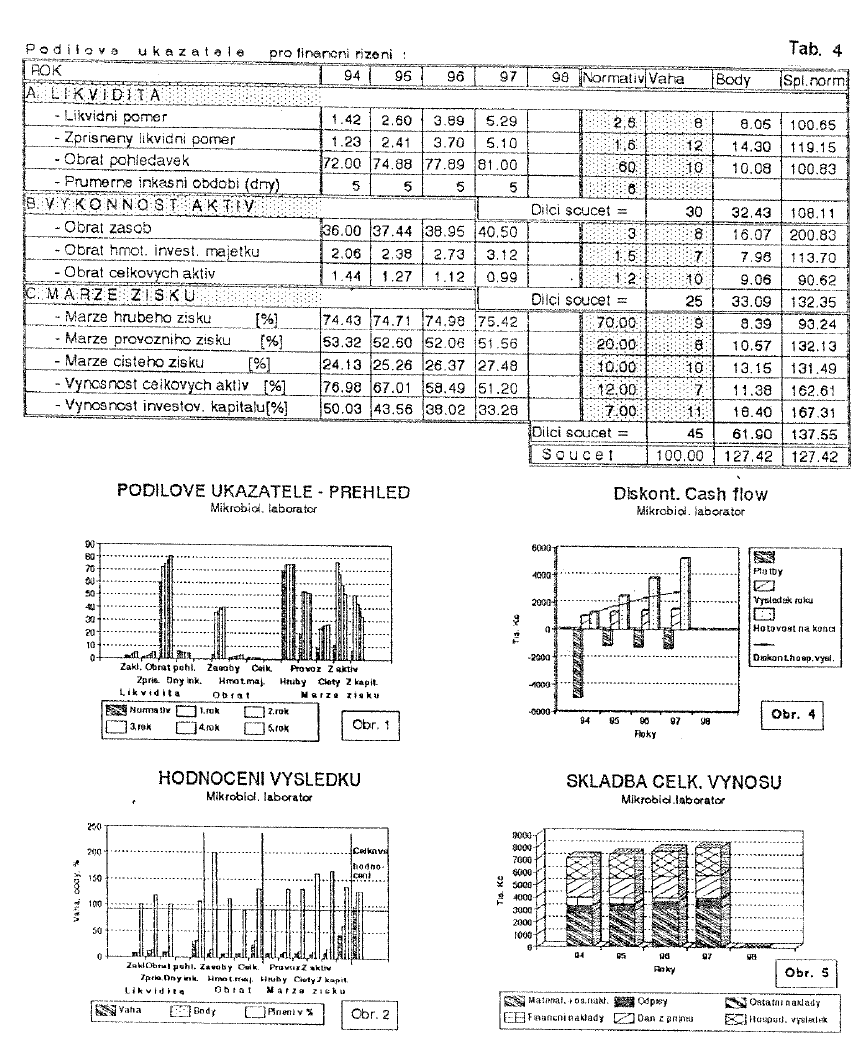
\includegraphics[width=\textwidth,height=\textheight,keepaspectratio]{./vesna3-obr2.png}

\newpage

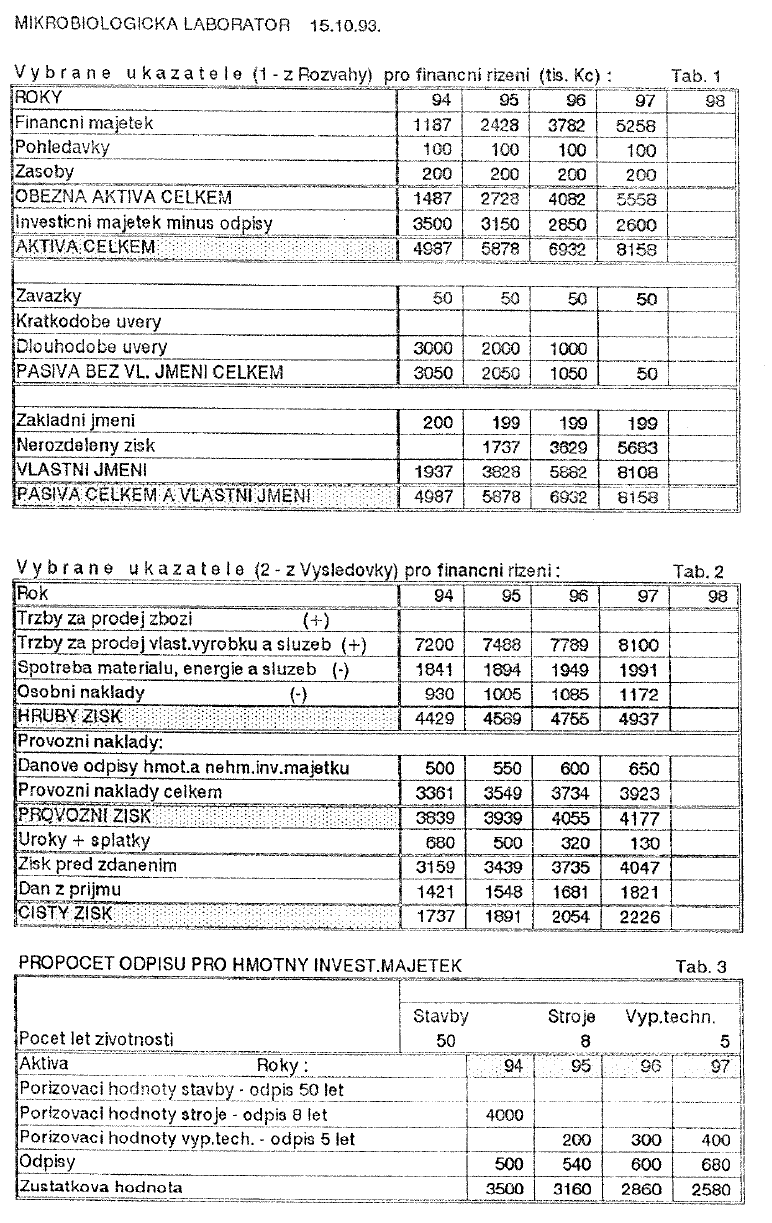
\includegraphics[width=\textwidth,height=\textheight,keepaspectratio]{./vesna3-obr3.png}




\end{document}
